
\textbf{Problem definition}

A quarter of an elastic cylinder is compressed at the top. The deformation that is caused by a uniform vertical stress is given as boundary condition. The aim is to calculate the stress in $z$-direction which is caused by this deformation and to get to know the resulting deformations in each direction.

\begin{figure}[htbp]
\centering
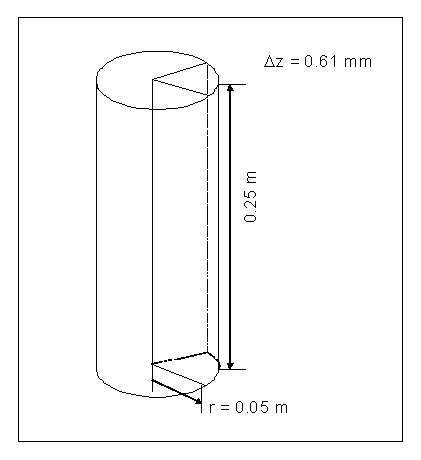
\includegraphics[width=0.4\textwidth]{M/figures/fig31.eps}
\caption{Calculation area: a quarter of a cylinder}
\label{fig31}
\end{figure}

%\newpage

\textsl{Assumptions}

\begin{tabbing}
\=xxxxxxxxxx  \=xxxxxxxxxxxxxxxxxxxxxxx \kill
\> Solid: \> homogeneous, isotropic, finite dimensions, constant deformation, \\
\> \> linear elastic material behaviour
\end{tabbing}

\textbf{Model set-up of the 3D numerical model}

For the 3-dimensional simulation the calculation area is exclusively out of a quarter of a cylinder. The model includes 4000 elements and 4947 nodes. Deformations in $x$-direction are suppressed in the $y-z$-plane. Deformations in $y$-direction are suppressed in the $x-z$-plane and deformations in $z$-direction are inhibited at the bottom of the quarter cylinder. At the top of the model a mechanical boundary condition is set with a constant displacement of 0.61~mm. The elastic deformation of the solid is not time-dependent. The used material parameters are shown in Tab. \ref{tab33}.
\begin{table}[htbp]
\centering
\begin{tabular}{|c|l|l|}
\hline
symbol & quantity & value \\
\hline
$\rho$  & density of the solid &  2.5 t$\cdot$m$^{-3}$  \\			
\hline
$E$ & Young's modulus of the solid & 7 GPa \\
\hline
$\nu$ & Poisson ratio & 0.3 \\
\hline
\end{tabular}
\caption{Material parameters}
\label{tab33}
\end{table}

\begin{figure}[htbp]
\centering
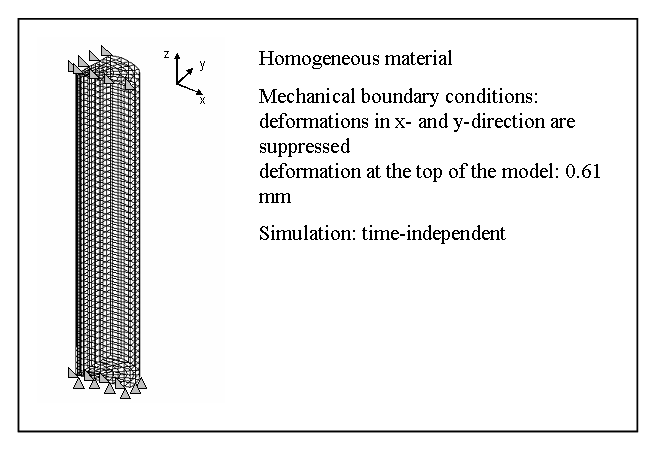
\includegraphics[width=0.5\textwidth]{M/figures/fig32.eps}
\caption{Calculation model (3D)}
\label{fig32}
\end{figure}

\newpage

\textbf{Evaluation method}

In order to solve the equations of the Hooke's law, there are some constraints that have to be considered: the stresses in $x$- and $y$-direction are equal to zero, because the body can expand into radial direction. Thus the Hooke's equations can be simplified as follows:
\begin{eqnarray}
\varepsilon_z & = &
\frac{\Delta z}{z}\,=\,\frac{1}{E}\cdot\sigma_z
\label{eq36} \\[1.5ex]
\varepsilon_x & = &
\varepsilon_x\,=\,\frac{1}{E}\cdot\left(-\nu\cdot\sigma_z\right)
\label{eq37}
\end{eqnarray}

\textbf{Results}

With the given strain in $z$-direction, the stress $\sigma_z$ is calculated by Eqn. \ref{eq36}.
\begin{displaymath}
\frac{\Delta z}{z}=\frac{-6.1\cdot 10^{-4}\,\mathrm{m}}{0.25\,\mathrm{m}}=-2.44\cdot 10^{-3}
\quad\mathrm{and}\quad
\sigma_z=-2.44\cdot 10^{-3}\cdot 7\cdot 10^{9}\,\mathrm{Pa}=
-1.71\cdot 10^{7}\,\mathrm{Pa}
\end{displaymath}

In this way, the strains in $x$- and $y$-direction are known.
\begin{displaymath}
\varepsilon_x\,=\,\varepsilon_y\,=\,
\frac{1}{7\cdot 10^{9}\,\mathrm{Pa}}\cdot
\left(-0.3\cdot-1.71\cdot 10^{7}\,\mathrm{Pa}\right)\,=\,
7.32\cdot 10^{-4}
\end{displaymath}

The numerical results meet exactly the analytical solutions. This is sketched in Fig. \ref{fig33}, where the strains and the resulting stress along a polyline from top to bottom of the quarter cylinder can be found. That means both RockFlow and GeoSys/RockFlow are able to calculate the state of stresses for the 3D elastic deformation.

\clearpage

\begin{figure}[htbp]
\centering
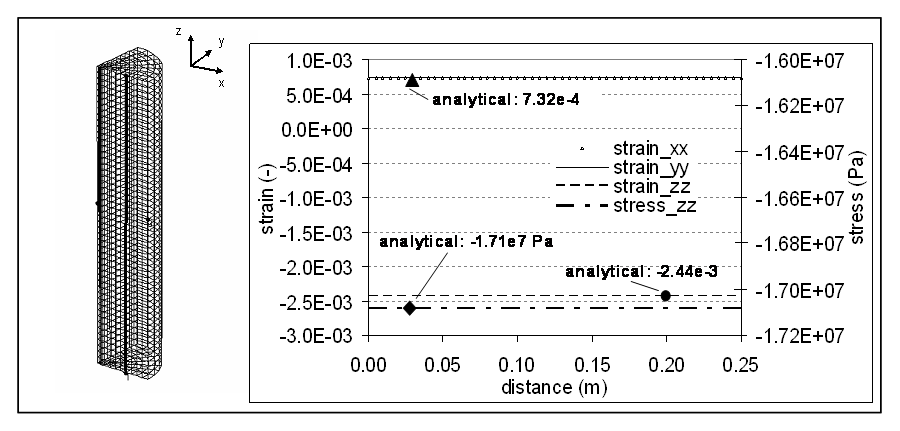
\includegraphics[width=0.9\textwidth]{M/figures/fig33.eps}
\caption{Strains and stress in $z$-direction as the result of deformation}
\label{fig33}
\end{figure}

\vskip 4.0ex

\begin{tabular}{|l|l|l|l|}
\hline
Path in the & Used code	& Used version & Date of si- \\
benchmark deposit	& & & mulation run \\
\hline	
$\backslash$M$\backslash$elastic\_deformation$\backslash$	& GeoSys/RockFlow	& RockFlow 4,	& Dec. 2007 \\
displacement$\backslash$displ\_Geosys/	& & rf4-507 & \\
RF$\backslash$m\_e\_displacement\_3Du	& & & \\
\hline	
\end{tabular}
